При заданном сдвиге по звёздной величине (или, что тоже самое, при заданном отношении усилений изображений) неопределённость во временной задержке, вызванная микролинзированием, не зависит от $\Delta t_{\textrm{ист.}}$. Отметим, что нормировочная постоянная $k$ в \eqref{chi2} по своему смыслу и есть заданная разница в блеске изображений.
%В действительности, в реально наблюдаемых изображениях гравитационно линзированных объектов нельзя точно указать отношение усилений, что нельзя не учитывать при более точных исследованиях. 
Для иллюстрации выбраны следующие значения временной задержки и разницы в звёздной величине: $$\Delta t_{\textrm{ист.}}=40, \ \Delta m = -0.28.$$
Для временных интервалов вводится равномерная сетка: частота отсчёта \textit{(cadence)} составляет $4$ дня. Модельная кривая блеска линейно интерполируется по этим точкам.
Сперва рассмотрим идеализированный случай, в котором наблюдение кривой блеска в обоих изображениях начинается с момента расширения сверхновой (Рис. \ref{fig:proba}a). В таком случае дисперсия очень маленькая: $\sigma_{\Delta t}=0.24$ дня. Это значение можно трактовать как нижнюю границу точности измерения временных задержек. Столь высокая точность объясняется следующими факторами: 

\begin{itemize}
    \item наличие характерной почти вертикальной части кривой блеска, обусловленной быстрым увеличением яркости сверхновой в первые дни после её взрыва,
    \item достаточно высокая частота отсчёта,
    \item погрешность измерения в формуле \eqref{chi2} относительно маленькая и постоянная.
\end{itemize}
Пусть теперь вертикальная часть охватывает меньший диапазон изменения блеска. В этом случае дисперсия резко возрастает и по порядку величины составляет несколько дней. ($\sigma_{\Delta t}=5.1$ дней, Рис. \ref{fig:proba}б). Если же ещё сильнее сдвинуть момент начала снятия кривой блеска, то дисперсия достигнет весьма больших значений ($\sigma_{\Delta t}=12.3$ дней, Рис. \ref{fig:proba}в). 


\begin{figure}[H]
    \centering
	\begin{minipage}[h]{1.0\linewidth}
    \centering    
    	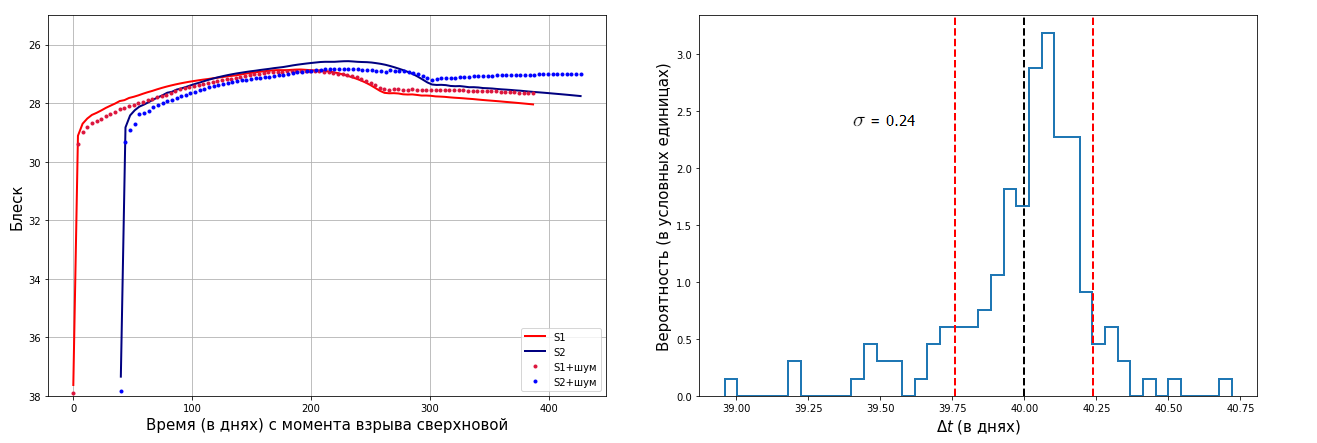
\includegraphics[scale=0.43]{pics/fig1.png} \\ \centering (а)  \\ 
	\end{minipage}
	\vfill
	\begin{minipage}[h]{1.0\linewidth}
	\centering
    	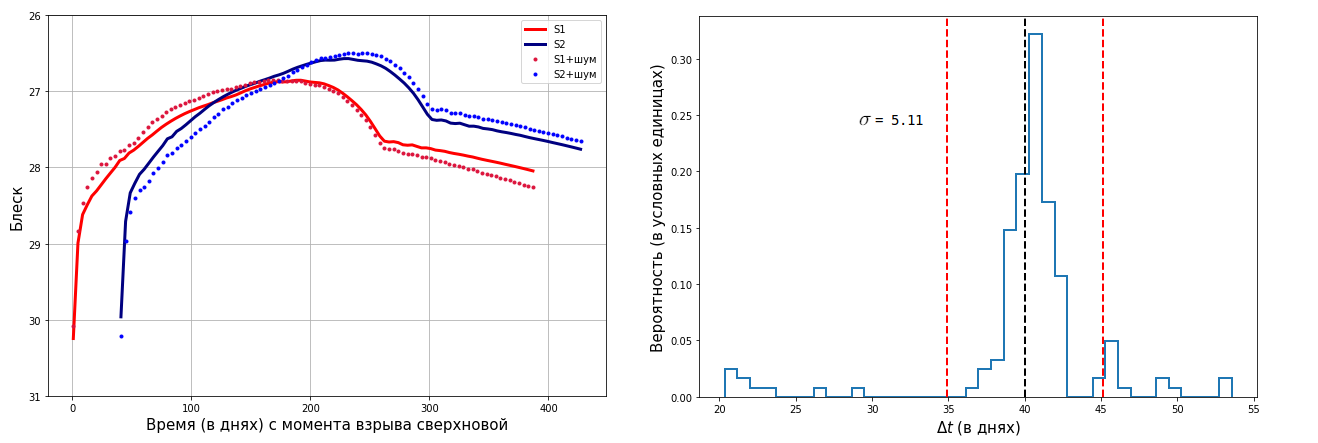
\includegraphics[scale=0.43]{pics/fig2.png} \\ \centering (б) \\
	\end{minipage}
	\vfill
	\begin{minipage}[h]{1.0\linewidth}
    \centering	
    	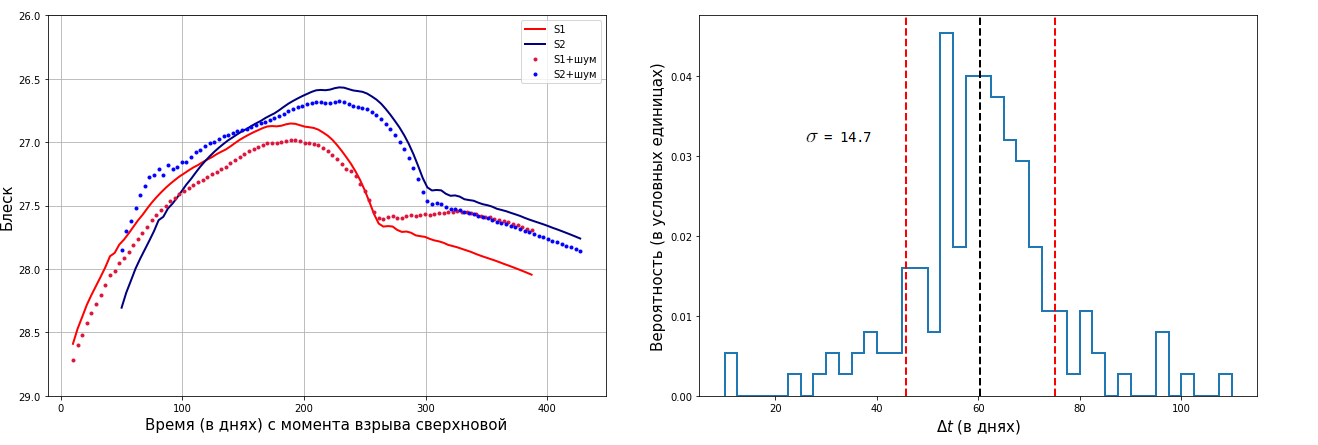
\includegraphics[scale=0.43]{pics/fig3.png} \\ \centering (в) \\
	\end{minipage}
	\vfill
	\begin{minipage}[h]{1.0\linewidth}
    \centering	
    	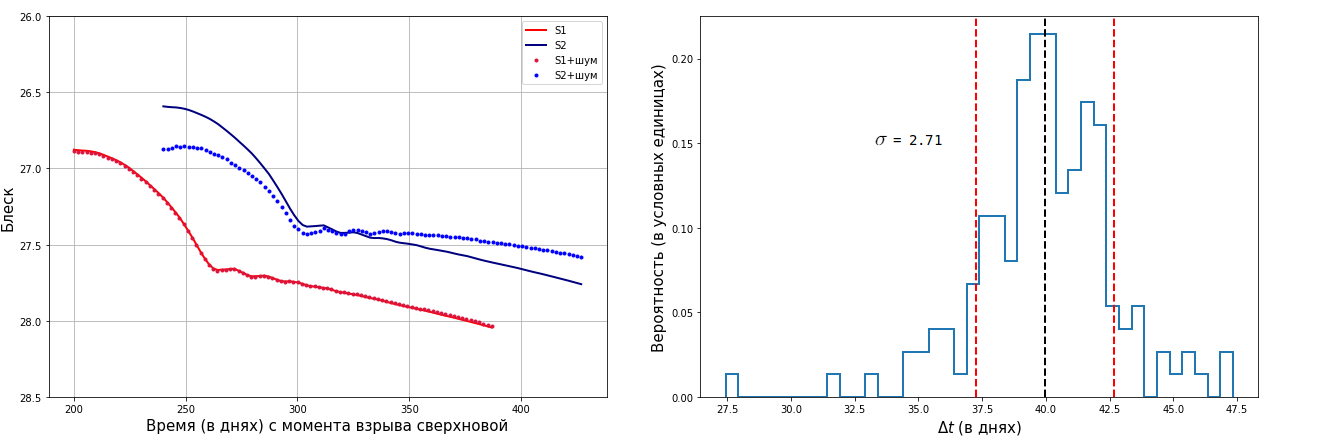
\includegraphics[scale=0.43]{pics/fig4.png} \\ \centering (г) \\
	\end{minipage}
	
	\caption{\textit{Слева}: кривые блеска в изображениях S1 и S2 SN Refsdal. Сплошной линией обозначены невозмущенные кривые блеска, точками -- одна из реализаций кривых блеска с шумами от микролинзирования, вносящими заметный вклад. \textit{Справа}: гистограммы временных задержек для 150 измерений $\Delta t$. Чёрной пунктирной линией обозначено среднее по всем измерениям, красными пунктирными линиями - среднее плюс-минус одно стандартное отклонение. \label{fig:proba}} 
\end{figure}
Теперь смоделируем ситуацию, когда сверхновая детектируется после достижения пика своего блеска. Для настоящих наблюдений сверхновых это наиболее реалистичная ситуация. В этом случае стандартное отклонение снова составляет несколько дней по порядку величины ($\sigma_{\Delta t}=2.7$ дней, Рис. \ref{fig:proba}г).

Несмотря на широкий разброс в значениях, данные согласуются с работой \cite{doblerkeeton2006} -- в ней также показано,  что флуктуации от микролинзирования наиболее сильно проявляются тогда, когда они совпадают по порядку величины с характерными изменениями истинной кривой блеска. Полученные результаты, однако, расходятся с выводами работы \cite{pierelrodney2019}, в которых утверждается, что для наблюдений кривой блеска сверхновой после её пика дисперсия временной задержки будет больше, чем для наблюдений с характерным пиком. Это расхождение, вероятнее всего, объясняется заданным и постоянным значением $\Delta m$. Дальнейшие исследования в этой области предполагают уточнение описанной модели.